\section{Introduction}
\label{sec:w-motiv}

Many financial instruments have been established and implemented in traditional fiat-based markets; 
among them: options, futures, loans, bonds, derivatives, etc. In the past decade, the concept of cryptocurrency has opened a new gate toward the next generation of economy and finance. This field is still open to new ideas and introduces lots of implementation challenges for DeFi. 

By the invention of Ethereum smart contracts, so many decentralized financial applications were built which have resulted in the rapid growth of the ether market capital in general, and the total value locked in liquidity and lending protocols specifically \new{\cite{aave, maker, compound, wbtc, dydx}}. This demonstrates the urgent need for the blockchain counterpart of well-known financial instruments, especially loans, options, and \emph{decentralized exchanges} (DEX), and as a result, DeFi primitives are being demanded these days more than ever before \new{\cite{buterin2014next, uniswap, flashswaps, jelly}}. 

In the present study, we tackle this challenge and design primitives for decentralized futures market applications which in addition to Ethereum blockchain, work on first-generation blockchains like Bitcoin which do not support high-level Turing-complete scripting languages. Our bond issuance system and the corresponding procedures only require \emph{hash time locked contracts} (HTLC) as their building block and they do not rely on any oracle or third party interference. To the best of our knowledge \abcd is the first protocol in DeFi which offers an atomic unsecured cross-chain bond service.

As the pioneer in decentralization, the pseudonymous Satoshi Nakamoto has devised a new path towards the peer-to-peer payment systems which are counted as a disruptive innovation today \new{\cite{nakamoto2019bitcoin}}. Ethereum as the next generation of decentralized computing services enables writing smart contracts on an electronic ledger \new{\cite{buterin2014next}}. Later on, by the advent of ever-increasing blockchains, one may need to exchange assets across different networks. Through utilizing atomic swaps, two parties on different blockchains make an atomic contract which transfers asset between them \new{\cite{htlc-btctalk}}. Up until now, several previous works have extended the usage of atomic swaps in different ways. Herlihy designed a model for analyzing atomic cross-chain swaps and suggested a protocol that not only removes incentives for any set of parties to deviate from the protocol, but also guarantees that no conforming party ends with the underwater outcome and showed that HTLCs are enough to achieved this \new{\cite{herlihy2018atomic}}. Zamyatin \etal presented X{\footnotesize CLAIM} which is a swap frame work based on the atomic swaps that is faster and considerably cheaper than normal atomic swaps \new{\cite{8835387}}.
% Meyden \etal considered the term of atomic swap multi-party transactions using smart contracts in \cite{van2019specification}.
The idea of atomic cross-chain transactions in Ethereum sidechains was developed in \new{\cite{robinson2019atomic}}. The conflict caused by the concurrent execution of smart contracts was addressed to make an all-or-nothing atomic cross-chain commitment protocol in \new{\cite{zakhary2019atomic}}. Furthermore, Runchao \etal put a step forth by analyzing the fairness of atomic swaps and showed that the basic atomic swap is considerably more unfair compared to its equivalent contracts in the traditional market. Besides, they proposed two enhanced atomic swap protocols and justified their fairness \new{\cite{10.1145/3318041.3355460}}.
% (1) if all parties conform to the protocol, then all swaps take place, (2) if some coalition deviates from the protocol, then no conforming party ends up worse off, and (3) no coalition has an incentive to deviate from the protocol.
Liu proposed an atomic swaption component which works only using low-level scripting tools \new{\cite{liu2018atomic}}. Additionally, by utilizing his swaption component, offering fully decentralized futures contracts is no longer impossible \new{\cite{liu2018atomic}}.
Zie~\etal extended the atomic cross-chain swap contracts to a new method that does not need HTLCs and everything is managed by different party's signatures \new{\cite{zie2019extending}}.
% Furthermore, we propose two fair Atomic Swap protocols, one is for currency exchange and the other is for American Call Options. The quantification results show that the the Atomic Swap is much more unfair on cryptocurrencies than on stocks and fiat currencies in the same setting. 


% Most of mentioned systems have one thing in common: they are implemented for a turing complete bock chain and with the aid of smart contracts.
% In order to show the economical willingness towards the subject, some financial application implementations are mentioned below:

% Some developed solutions for applying these traditional economical applications to the world of crypto-currencies are:

% Some of the reputed DeFi applications are Compound, Maker DAO

% There are some developed solutions for applying these traditional economical applications to the world of crypto-currency.Here are some examples from


% \begin{itemize}
%     \item \textbf{ACO}: A protocol for decentralized and non-custodial trading of options \cite{aco}.
%     \item \textbf{Jelly Swap}: A peer to peer trading tool across different blockchains using atomic swaps \cite{jelly}.
%     \item \textbf{Uniswap}: A fully decentralized on-chain protocol for token exchanges on Ethereum that uses liquidity pools instead of order books \cite{uniswap}.
%     \item \textbf{Aave}: An open source and non-custodial protocol to earn interest on depositing and borrowing assets \cite{aave}.
%     \item \textbf{MakerDAO}: A decentralized credit platform on Ethereum that supports Dai, a stablecoin whose value is pegged to USD and backed in ETH or BAT \cite{maker}. 
%     \item \textbf{Compound}: An open-source money market protocol on Ethereum that lets users lend or borrow assets against collateral \cite{compound}. 
%     \item \textbf{Atomic Loan}: A lending platform that accepts trustless BTC collateral via custom Bitcoin scripts \cite{atomicLoan}. 
%     \item \textbf{DAI}: A decentralized stablecoin soft-pegged to the US Dollar \cite{maker}. 
%     \item \textbf{WBTC}: An ERC20 token that is backed 1:1 by bitcoin and opened the gate of trading bitcoin under ethereum blockchain \cite{wbtc}.
%     \item \textbf{dYdX}: An non-custodial trading platform on Ethereum geared toward experienced traders \cite{dydx}. 
    
% \end{itemize}

% For showing the growing investment interest in financial derivatives of crypto currencies, we can consider Fig.~\ref{fig:TVL-ACO} and \ref{fig:TVL-Uniswap} which are the overview of the money (in USD) locked in Uniswap and ACO and their fluctuations during the recent three months:
% \begin{figure}
%     \centering
%     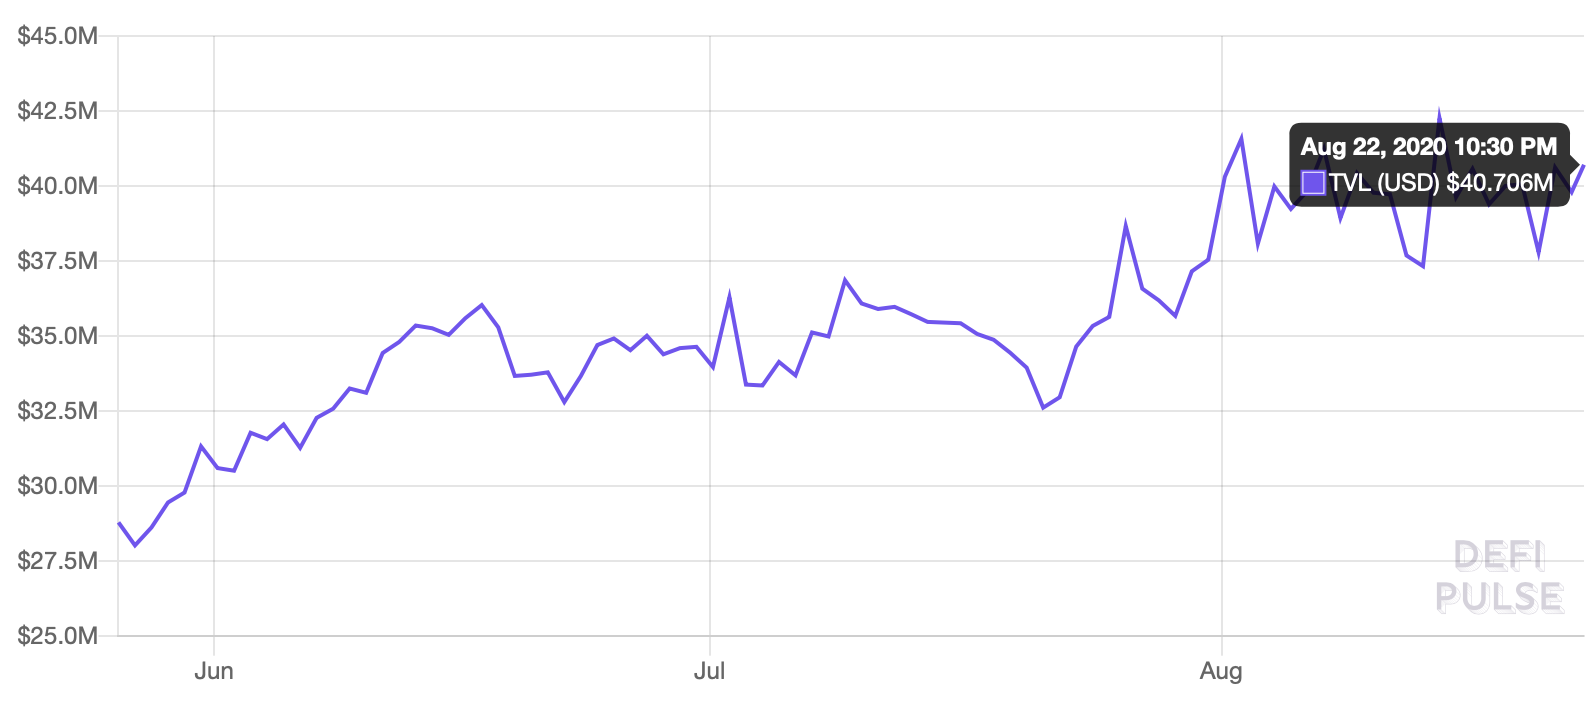
\includegraphics[width=\textwidth]{figures/dydx.png}
%     \caption{Total value locked (USD) in dydx \cite{dydx-cap}. Currently more than 40 M\$}
%     \label{fig:TVL-ACO}
% \end{figure}
% \begin{figure}
%     \centering
%     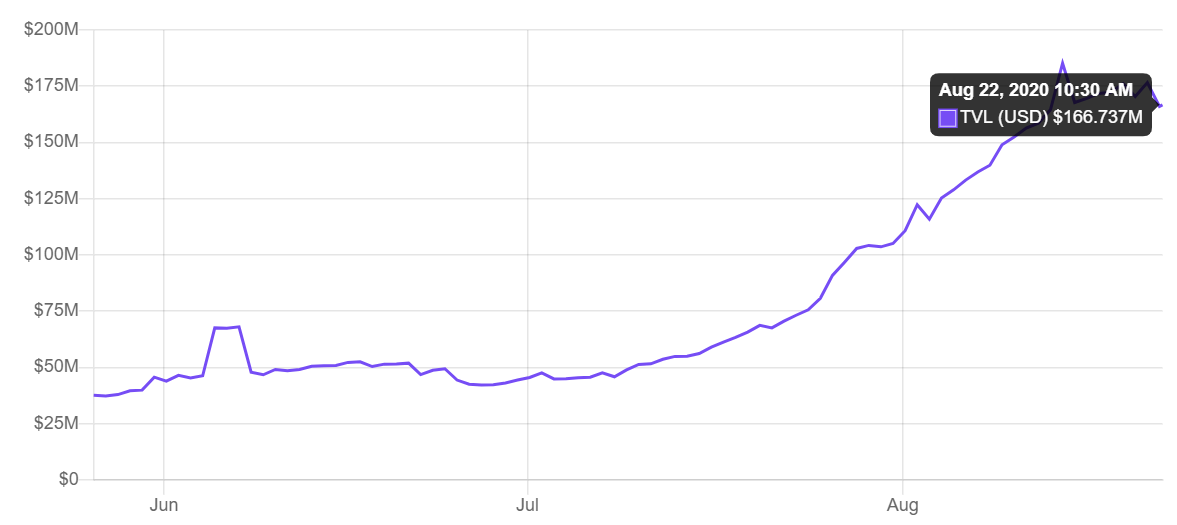
\includegraphics[width=\textwidth]{figures/TVL(USD)-uniswap-90.png}
%     \caption{total value locked (USD) in Uniswap \cite{uniswap-cap}. Currently more than 166 M\$}
%     \label{fig:TVL-Uniswap}
% \end{figure}





% \begin{tabular}{||c c c c c c||} 
%  \hline
%  BTC & ETH & DAI & AE & WBTC & USDC \\ [0.5ex] 
%  \hline\hline
%  20709.97 & 19216.02 & 9598.86 & 10226.57 & 209.33 & 3756.75 \\ [1ex] 
%  \hline
% \end{tabular}


 
The rest of this paper is organized as follows. First of all, in section~\ref{sec:abd} after defining the required terminology and presenting the other preliminaries of our work, we introduce the first \newfateme{model} of atomic bonded debt \newfateme{and discuss about the crucial requirements of an atomic bond service.} Later in section~\ref{sec:abcd}, we redesign our model to build the first practical \emph{atomic bonded cross-chain debt} (ABCD) primitive, \newfateme{and finally by adding additional features to it, we improve its stability across different market behaviours.}


% by using it afterwards, we build the \new{\emph{atomic bonded cross-chain debt} primitive (ABCD)}. 
% first practical version of ABCD component. Finally in the section~\ref{sub:seq-bond} we modify the ABCD to be used in the scenario of cross chain usecase.
% In Section~\ref{sec:relatedWorks}, we review some of the most important and recent studies on traffic classification with details. In Section~\ref{sec:Background}, we present the essential background on machine learning used in proposed methods, including deep learning and decision tree. In Section~\ref{sec:dataset}, we discuss the process of dataset collection and its various aspects, \eg, the reason for using two different datasets. Section~\ref{sec:Methodology} presents our proposed iterative procedure and the details of employed classifiers. The results of our experiments on the gathered data are elaborated in Section~\ref{sec:results}. Finally, we conclude the paper in Section~\ref{sec:conc}, briefing what we have learned throughout this study and how to improve it further.

